

\documentclass[12pt]{article}

\usepackage{amsmath}
\usepackage{amsfonts}
\usepackage{amssymb}
\usepackage{amsthm}
\usepackage{graphicx}
\usepackage{stmaryrd}

\usepackage{cite}
\usepackage{caption}
\usepackage{url}
\usepackage{color}\usepackage{placeins}
\usepackage{svg}

\usepackage{accents}
\usepackage{algorithm}
\usepackage{algpseudocode}
\usepackage{mathtools}
\usepackage{subcaption}
\usepackage{multirow}
\usepackage{bbm}
\usepackage{epstopdf}
\usepackage{graphicx}
\usepackage{bm}
\usepackage{enumerate}
\usepackage{booktabs}
\usepackage[normalem]{ulem}

\theoremstyle{definition}\newtheorem{lemma}{Lemma}
\newtheorem{theorem}{Theorem}
\newtheorem{corollary}{Corollary}
\newtheorem{definition}{Definition}
\newtheorem{remark}{Remark}
\newtheorem{example}{Example}
\newcommand{\norm}[1]{\left\lVert#1\right\rVert}
\newcommand\Tstrut{\rule{0ex}{2.7ex}}         % = `top' strut
\newcommand\Bstrut{\rule[-1.3ex]{0pt}{0pt}}   % = `bottom' strut
\newcommand\Strut{\rule{0ex}{0ex}}         % = `top' strut
\newcommand\e{\textrm{e}}
\newcommand\m{\textrm{m}}
\newcommand\bt{\textrm{b}}



\renewcommand{\i}{{\mathrm{i}}}
\DeclareMathOperator*{\argmax}{arg\,max}
\DeclareMathOperator\supp{supp}
\DeclareMathOperator\erfc{erfc}

\algdef{SE}{Begin}{End}{\textbf{begin}}{\textbf{end}}

\topmargin -0.7in 
\oddsidemargin -0.25in 
\textheight 9.2in 
\textwidth 7.0in 

\title{Solving the Self-Similar Burgers Equation 
via Chebyshev Collocation and Gradient-Based Optimization}

\author{Allen Yang}

\begin{document}
\maketitle
\noindent\textit{Textbook Chapter}: Chapter 10, Boundary Value Problems for ODEs;\\
\textit{Contribution of the Authors}: Worked by myself;\\
\textit{Use of AI tools}: I used AI tools to help with code development, generating ideas, and writing the final report;\\
\textit{Other Sources}: I consulted with Prof. Koumoutsakos to discuss approaches for the problem of inferring the parameter $\lambda$.
\newpage
\section{\label{sec:introduction}Introduction}
Finite time self-similar blowups are a fundamental phenomenon in the study of nonlinear partial differential equations, especially in the context of fluid dynamics and nonlinear evolution equations such as the Navier-Stokes equations. A \textit{blowup} refers to the formation of a singularity in finite time, where the solution (or its derivatives) becomes unbounded as some critical time is approached.

In a \textit{self-similar blowup}, the solution near the singularity exhibits a structure that is invariant under a specific scaling of space and time. 
That is, as the singularity is approached, the solution can often be represented in terms of a single similarity variable—a specific combination of space and time.
This allows one to seek solutions of the PDE in a reduced form, often involving similarity variables, which convert the original problem into an ordinary differential equation (ODE) or a simpler PDE.

One of the simplest PDEs which exhibits self-similar blowups is the inviscid Burgers equation,
\begin{equation}
u_t + u u_x = 0,
\end{equation}
in which smooth initial conditions can develop a singularity in finite time. Taking the local self-similar ansatz
\begin{equation}\label{eq:self-similar-ansatz}
    u(x, t) = (1-t)^\lambda U(y(x, t)), \quad y(x, t) = \frac{x}{(1-t)^{1+\lambda}},
\end{equation}
the self-similar Burgers equation becomes
\begin{equation}
    -\lambda U + ((1+\lambda)y +U)d_yU = 0,
\end{equation}
which is a first order nonlinear ODE for $U(y)$. If we additionally impose $U$ to be odd and add the boundary conditions $U(-2) = 1$ and $U(2) = -1$, then the analytical self-similar Burgers' solution is given (implictly) by:
\begin{equation}\label{eq:solution}
    y = -U - CU^{1+\tfrac{1}{\lambda}}.
\end{equation}
Thus, for this project, we consider the boundary value problem
\begin{equation}\label{eq:bvp}
    \begin{cases}
        -\lambda U + ((1+\lambda)y +U)d_yU = 0, \quad y \in (-2, 2), \\
        U(-2) = 1, \quad U(2) = -1.
    \end{cases}
\end{equation}
To understand blowup in this context, notice that the spatial derivative transforms as $\partial_x u = (1-t)^{-\lambda} d_y U$ under the self-similar ansatz. This means if $d_y U$ is nontrivial, then as $t \to 1^-$, the factor $(1-t)^{-\lambda}$ diverges for any $\lambda > 0$, leading to a blowup in the gradient of $u(x, t)$. At the initial time $t=0$, the similarity variable reduces to $y(x, 0) = x$, so if $U(y)$ is smooth within $y \in (-2, 2)$, then $u(x, 0)$ is smooth for $x \in (-2, 2)$. As time advances towards $t = 1$, the region described by the fixed ``inner region'' $y \in [-2, 2]$ corresponds to an increasingly small neighborhood around $x = 0$, capturing precisely where the gradient becomes unbounded. Thus, the primary objective is to find a smooth solution $U(y)$ to the boundary value problem~\eqref{eq:bvp}, which allows us to clearly demonstrate how smooth initial conditions can evolve into a finite-time singularity. 
We focus on the inviscid Burgers equation due to its well-understood analytical properties, particularly the existence of an explicit self-similar solution~\eqref{eq:solution}, as well as the discrete set of parameter values $\lambda$ admit smooth solutions to the boundary value problem, given by
\begin{equation}
    \lambda = \frac{1}{2(j+1)}, \qquad j = 0, 1, 2, \ldots.
\end{equation}
For other $\lambda$, the solutions demonstrate nonsmooth behavior at $y=0$.

Related work done in~\cite{wang2023asymptotic} demonstrates the application of Physics-Informed Neural Networks (PINNs) to the self-similar Burgers equation problem. In their approach, they parameterize the solution $U(y)$ using a neural network and incorporate the PDE residual from~\eqref{eq:bvp} directly into the loss function. The network is trained to minimize a weighted combination of the PDE residual, boundary conditions, and additional regularization terms. Both their method and the approach used in this project rely on automatic differentiation for efficient evaluation of derivatives and gradients. However, while~\cite{wang2023asymptotic} uses neural networks as the ansatz space, this project employs a variation of the Chebyshev collocation method (cf.~\cite{driscoll2016rectangular}), which can achieve spectral accuracy for smooth solutions, also using automatic differentiation for gradient-based optimization. 

The remainder of this report is organized as follows. Section~\ref{sec:fixed_l} introduces the localized Chebyshev collocation method used to discretize the boundary value problem~\eqref{eq:bvp} and presents numerical experiments that demonstrate the accuracy and efficiency of this spectral discretization for fixed, known values of $\lambda$. In Section~\ref{sec:inference}, we turn to the more challenging problem of inferring the parameter $\lambda$ for which the ODE~\eqref{eq:bvp} admits a smooth solution $U$, and we formulate and solve the resulting coupled optimization problem. Finally, Section~\ref{sec:conclusions} summarizes the key findings of the project and outlines furture directions.

\section{\label{sec:fixed_l}Solving for fixed $\lambda$}
\subsection{Localized Chebyshev collocation}\label{subsec:collocation}

For values of $\lambda$ that are not exactly equal to $\lambda = 1/(2(j+1))$ for $j = 0, 1, 2, \ldots$, the solution $U(y)$ to~\eqref{eq:bvp} exhibits nonsmooth behavior at the origin. For this project we specifically consider $\lambda$ in a neighborhood of $\lambda=0.5$, where the fourth derivative $U^{(4)}(y)$ becomes unbounded as $y \to 0$ for $\lambda \neq 0.5$. This nonsmoothness poses a challenge for standard spectral methods, which assume global smoothness of the solution. 
To overcome this, we utilize a localized Chebyshev collocation approach by dividing the domain $[-2, 2]$ into two subintervals: $[-2, 0]$ and $[0, 2]$, and discretize each segment with Chebyshev points, which naturally cluster near the boundaries of each segment. More concretely, for a given (even) resolution parameter $n_y$, we divide the domain $[-2, 2]$ into two subintervals, $[-2, 0]$ and $[0, 2]$. Each subinterval is discretized using $n_y/2 + 1$ Chebyshev collocation points, resulting in a total of $n_y + 1$ distinct points overall—-with the endpoint $y = 0$ shared by both subintervals. For the remainder of this report, we denote
\begin{equation}
    Y_1 = \{-2=y_0, y_1, \ldots, y_{n_y/2}=0\}\subset [-2, 0]
\end{equation}
and
\begin{equation}
    Y_2 = \{0=y_{n_y/2}, y_{n_y/2+1}, \ldots, y_{n_y}=2\} \subset [0, 2].
\end{equation}
to be the sets of Chebyshev collocation points in ascending order for the two subintervals, and subsequently, for a given profile $U$, we define
\begin{equation}\label{eq:U_1_U_2}
    \mathbf{U}_1 = (U(y_0), \ldots, U(y_{n_y/2}))^t \in \mathbb{R}^{n_y/2+1} \quad \text{and} \quad \mathbf{U}_2 = (U(y_{n_y/2}), \ldots, U(y_{n_y}))^t \in \mathbb{R}^{n_y/2+1}.
\end{equation}
The corresponding derivative vectors $D\mathbf{U}_1 \in \mathbb{R}^{n_y/2+1}$ and $D \mathbf{U}_2 \in \mathbb{R}^{n_y/2+1}$ can then be computed via spectral differentiation, and, further, higher order derivatives can be obtained analogously through repeated application of the derivative operator.
\begin{remark}
    For notation clarity, the rest of the report uses zero indexing for vectors, e.g. $\mathbf{U}_1 $ in \eqref{eq:U_1_U_2} can equivalently be written as $\mathbf{U}_1 = ((\mathbf{U}_1)_0, (\mathbf{U}_1)_1, \ldots, (\mathbf{U}_1)_{n_y/2})^t \in \mathbb{R}^{n_y/2+1}$.
\end{remark}

On each open segment $(-2, 0)$ and $(0, 2)$, the solution $U$ remains smooth, allowing the spectral method to accurately capture its behavior within each piece. 
This clustering property is also intuitive: because $y=0$ serves as the shared interface between the two subintervals, the Chebyshev points naturally accumulate near this nonsmooth region. As a result, we achieve enhanced resolution precisely where the solution demands finer discretization, allowing for more accurate representation and treatment of the challenging behavior near the origin. The advantage of this approach is illustrated in Figure~\ref{fig:deriv_comparison}, which compares the fourth derivative computed using three different methods: regular Chebyshev collocation on the full domain, localized Chebyshev collocation, and first-order finite differences. The plot clearly demonstrates that the localized method provides superior accuracy near the origin, where the fourth derivative becomes unbounded. The regular Chebyshev method struggles to capture this behavior due to its global smoothness assumption, while the localized approach naturally clusters points around the nonsmooth region, providing the necessary resolution to accurately represent the solution structure.

\begin{figure}[tbhp]
    \centering
    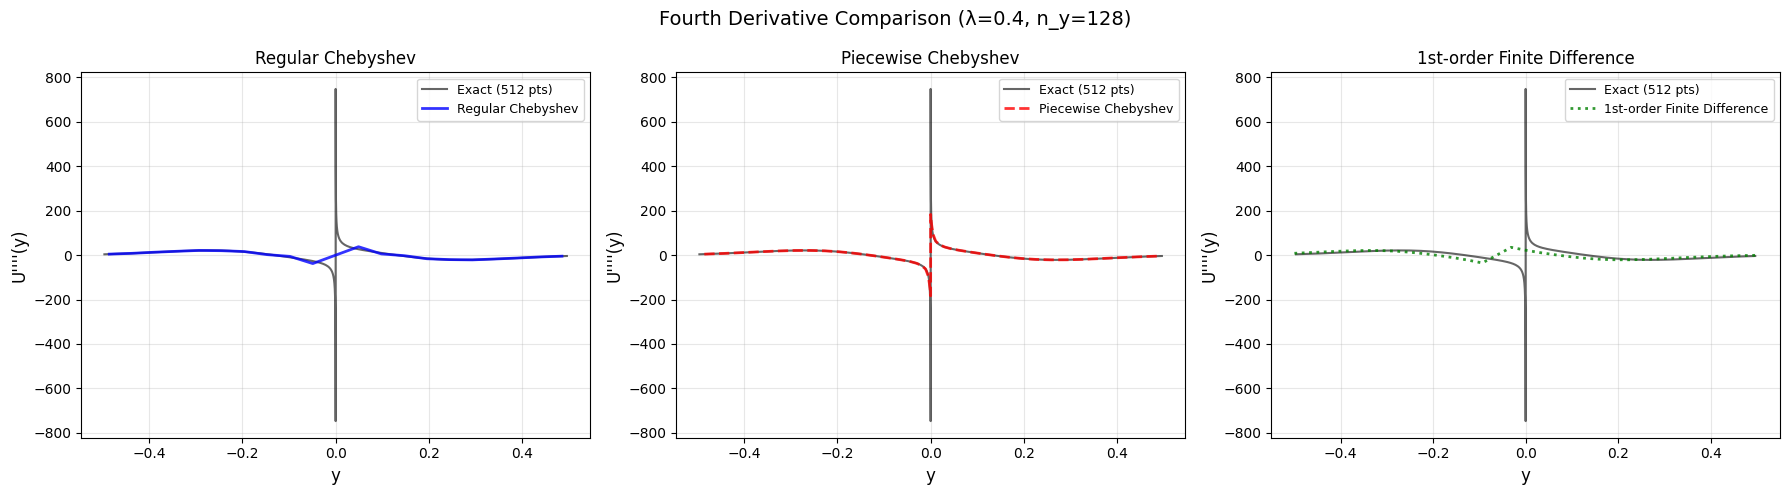
\includegraphics[width=\textwidth]{images/deriv_exact_comparison.png}
    \caption{Comparison of fourth derivative $U^{(4)}(y)$ computed using different differentiation methods for $\lambda = 0.4$ and $n_y = 128$ discretization points. The exact solution (black line) is computed using spectral differentiation with 512 points. The plot demonstrates that the localized Chebyshev method provides superior accuracy near the origin, where the fourth derivative becomes unbounded.}
    \label{fig:deriv_comparison}
\end{figure}

\subsection{Objective function and optimization}\label{subsec:optimization}

Rather than minimizing a weighted loss function that combines PDE residuals and boundary conditions as in the PINNS setting introduced in~\cite{wang2023asymptotic}, we formulate the problem as the root-finding of a certain vector function $\mathcal{L}_\lambda: \mathbb{R}^{n_y/2+1} \times \mathbb{R}^{n_y/2+1} \to \mathbb{R}^{n_y+2}$ where $n_y$ is the resolution parameter introduced in the preceding section. In detail, for a given $\lambda$, the vector function $\mathcal{L}_\lambda(\mathbf{U}_1, \mathbf{U}_2)$ is given by 
\begin{equation}\label{eq:fixed_l_loss}
    \mathcal{L}_\lambda(\mathbf{U}_1, \mathbf{U}_2) = 
    \begin{pmatrix}
        \mathcal{L}^{\textrm{PDE}}_\lambda(\mathbf{U}_1)\\
        \mathcal{L}^{\textrm{PDE}}_\lambda(\mathbf{U}_2)\\
        \mathcal{L}^{\textrm{BC}}_\lambda(\mathbf{U}_1,\mathbf{U}_2)\\
        \mathcal{L}^{\textrm{interface}}_\lambda(\mathbf{U}_1, \mathbf{U}_2)\\
    \end{pmatrix}
\end{equation}
where
\begin{equation}
    (\mathcal{L}^{\textrm{PDE}}_\lambda(\mathbf{U}))_{i-1} = -\lambda (\mathbf{U})_i + ((1+\lambda)y_i + (\mathbf{U})_i)(D\mathbf{U})_i, \quad i = 1, 2, \ldots, n_y/2-1,
\end{equation}
\begin{equation}
    (\mathcal{L}^{\textrm{BC}}_\lambda(\mathbf{U}_1,\mathbf{U}_2))_{i} = 
    \begin{cases}
        (\mathbf{U}_1)_0 - 1, & i = 0, \\
        (\mathbf{U}_2)_{n_y/2} - 1, & i = 1, \\
    \end{cases}
\end{equation}
and
\begin{equation}
    (\mathcal{L}^{\textrm{interface}}_\lambda(\mathbf{U}_1, \mathbf{U}_2))_{i} = 
    \begin{cases}
        (\mathbf{U}_1)_{n_y/2} - (\mathbf{U}_2)_{0}, & i = 0, \\
        (D\mathbf{U}_1)_{n_y/2} - (D\mathbf{U}_2)_{0}, & i = 1.
    \end{cases}
\end{equation}
In summary, these residuals enforce the boundary value problem within each subinterval, while simultaneously imposing continuity and flux matching conditions at the interface $y = 0$. This ensures both the solution and its first derivative are properly matched at the subdomain boundary, capturing the essential coupling between the two regions.

To solve this system, we employ Newton-type methods (specifically, Powell's hybrid method) with the Jacobian computed exactly using automatic differentiation via JAX. Because convergence to the correct solution becomes more delicate at higher resolutions (larger $n_y$), we employ a multigrid-style strategy for constructing initial guesses. We first solve the system on a coarse grid, interpolate the solution onto a finer grid using piecewise linear interpolation, and use this interpolated solution as the initial guess for the solver at the increased resolution. Iterating this process from coarse to fine grids provides high-quality initial guesses, greatly improving convergence and robustness of the solver.

\subsection{Fixed $\lambda$: numerical results}\label{subsec:fixed_l_numerical_results}
In this section, we present the effectiveness of the proposed method for solving the boundary value problem~\eqref{eq:bvp} for a fixed $\lambda$. We consider the non-smooth case where $\lambda = 0.4$ and the smooth case where $\lambda = 0.5$, using a discretization of $n_y = 64$ for the numerical solution. Figure~\ref{fig:fixed_l} displays the numerical solution $U(y)$ and its first four derivatives $U'(y)$, $U''(y)$, $U'''(y)$, and $U^{(4)}(y)$ for both values of $\lambda$. The numerical solutions (blue solid lines) are obtained using the localized Chebyshev collocation method described in Section~\ref{subsec:collocation} and the root-finding approach with Powell's hybrid method from Section~\ref{subsec:optimization}, where the Jacobian is computed using automatic differentiation. The exact solutions (red dashed lines, see eq.~\eqref{eq:solution}) serve as reference. 
The derivative of the exact solution are computed via the spectral differentiation method with the localized Chebyshev nodes described in Seciton~\ref{subsec:collocation} using the finer resolution $n_y = 128$. In view of the rapid convergence of spectral differentiation for smooth functions, the approximation error becomes negligible relative to the error for the coarser resolution $n_y = 64$.
Finally, we optimize to a tolerance of $10^{-9}$ and use multigrid levels $n_y = 2, 4, 8, 16,$ and $32$ for constructing initial guesses via piecewise linear interpolation.

\begin{remark}\label{rmk:n_y-selection}
    We found that choosing $n_y = 64$ consistently produced the most accurate results across the first four derivatives. Smaller values of $n_y$ were unable to adequately resolve the solution, while larger values led to differentiation matrices with prohibitively large condition numbers. For these reasons, all numerical experiments in this report use the choice $n_y = 64$.
\end{remark}

In both cases, we observe that the numerical solution is in good agreement with the exact solution. For the case $\lambda = 0.4$, we observe an absolute $\ell_\infty$ error of $2.1 \times 10^{-7}$ and a relative $\ell_2$ error of $1.2 \times 10^{-7}$, while for the case $\lambda = 0.5$, we observe an absolute $\ell_\infty$ error of $1.7 \times 10^{-7}$ and a relative $\ell_2$ error of $1.1 \times 10^{-7}$. The solution $U(y)$ itself is smooth and well-captured, with the numerical method accurately reproducing the odd symmetry and boundary conditions $U(-2) = 1$ and $U(2) = -1$. The interface conditions at $y = 0$—requiring continuity of both the solution and its first derivative—are also successfully recovered through the system formulation, as evidenced by the smooth transition visible in the plots. 
Although the numerical higher order derivatives (particularly the third and fourth) show instabilities near the boundaries, the method nevertheless resolves the key features distinguishing the two solutions: the cusp at the origin when $\lambda = 0.4$ and the smooth profile for $\lambda = 0.5$, achieving accuracies comparable to the PINN-based method reported in~\cite{wang2023asymptotic}. Further, the multigrid strategy employed for constructing initial guesses demonstrates efficient convergence behavior as shown in Table~\ref{tab:iterations}, typically requiring between 4 and 35 Newton iterations per level. Notably, the iteration count does not grow dramatically with increasing resolution, indicating that the piecewise linear interpolation between grid levels provides high-quality initial guesses that significantly accelerate convergence. We also note that in general, the smooth case ($\lambda = 0.5$) generally requires fewer iterations at intermediate levels compared to the non-smooth case ($\lambda = 0.4$).

Overall, the results demonstrate that the localized Chebyshev collocation method, combined with gradient-based optimization, provides an effective and accurate approach for solving the boundary value problem~\eqref{eq:bvp}, even in the presence of non-smooth behavior at the origin. The method successfully handles both smooth and non-smooth cases, with the natural clustering of Chebyshev points near the origin ensuring adequate resolution where it is most needed.

\begin{figure}[tbhp]
    \centering
    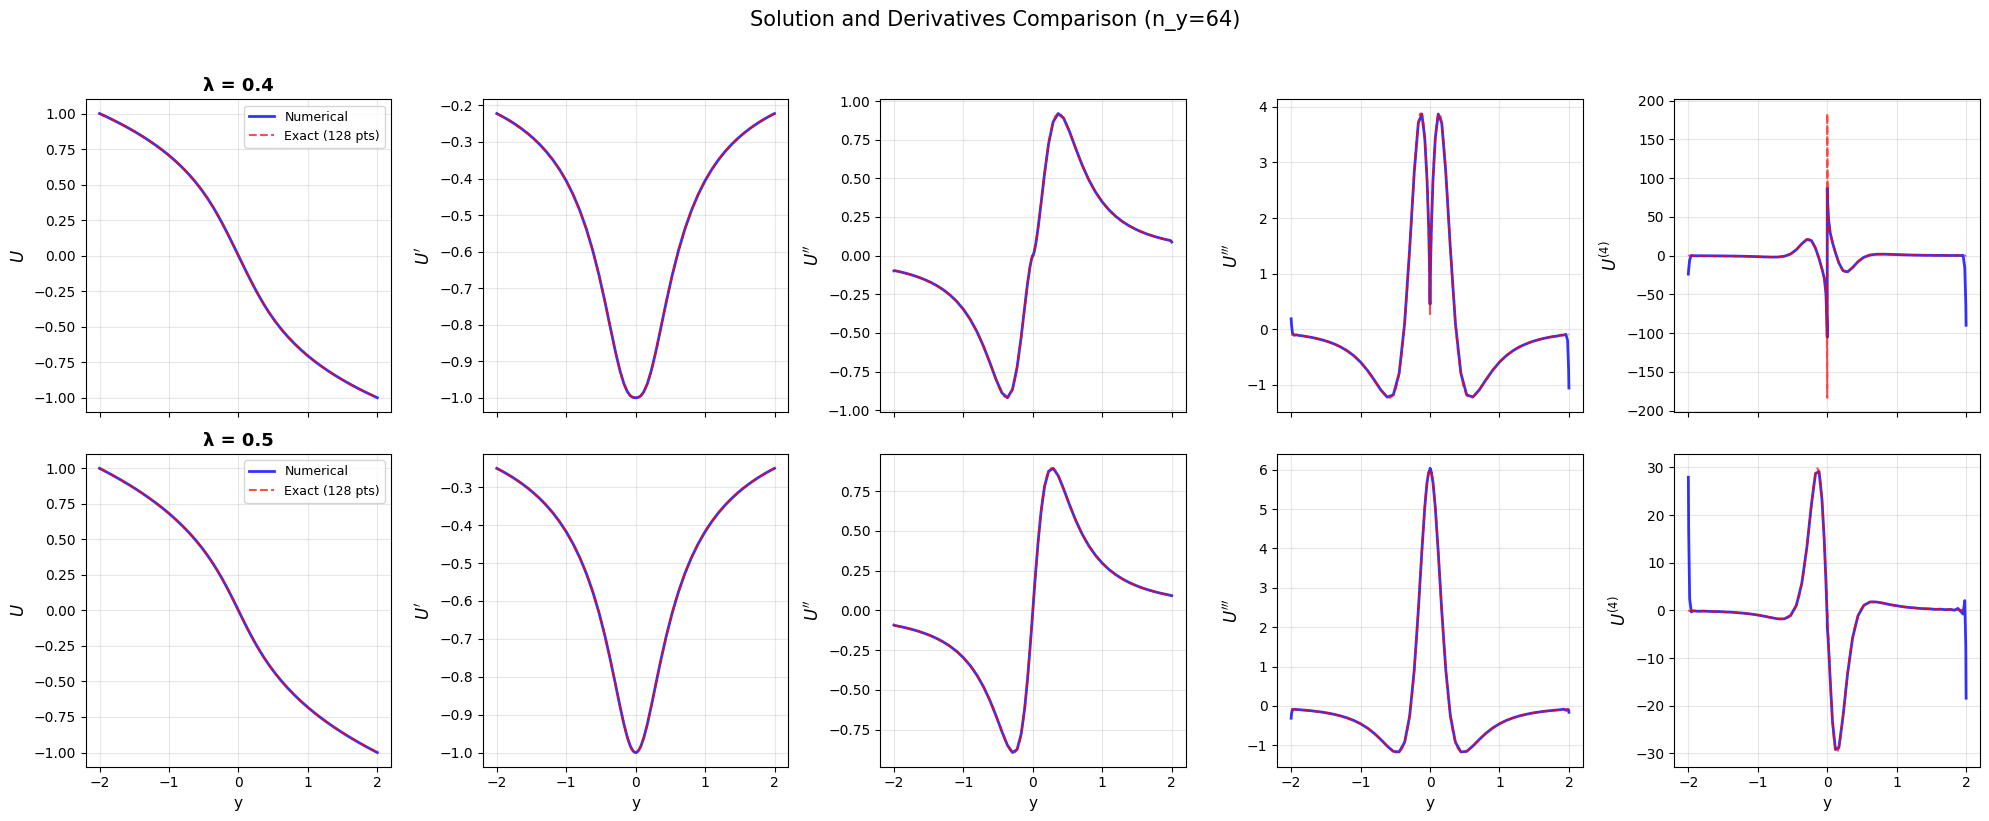
\includegraphics[width=\textwidth]{images/fixed_l.png}
    \caption{Comparison of numerical solutions (blue solid lines, $n_y = 64$) and exact solutions (red dashed lines) for the boundary value problem~\eqref{eq:bvp} with $\lambda = 0.4$ (top row) and $\lambda = 0.5$ (bottom row). Each row displays the solution $U(y)$ and its first four derivatives. The numerical method accurately captures both the smooth case ($\lambda = 0.5$) and the non-smooth case ($\lambda = 0.4$), where the fourth derivative becomes unbounded near the origin.}
    \label{fig:fixed_l}
\end{figure}


\begin{table}[tbhp]
    \centering
    \begin{tabular}{c|c|c}
        \toprule
        $n_y$ & Iterations ($\lambda = 0.4$) & Iterations ($\lambda = 0.5$) \\
        \midrule
        2 & 5 & 5 \\
        4 & 14 & 4 \\
        8 & 20 & 22 \\
        16 & 20 & 22 \\
        32 & 35 & 30 \\
        64 & 26 & 18 \\
        \bottomrule
    \end{tabular}
    \caption{Newton iteration counts for multigrid levels considered in Section~\ref{subsec:fixed_l_numerical_results}. We can see the multigrid strategy is effective in providing high-quality initial guesses, as iteration counts do not grow dramatically with increasing resolution.}
    \label{tab:iterations}
\end{table}

\section{\label{sec:inference}Inferring $\lambda$}
\subsection{Objective function and optimization}\label{subsec:inference_optimization}
As mentioned in the preceding sections, our goal is to single out the smooth solution at $\lambda = 0.5$ from nearby non-smooth solutions by exploiting the fact that the non-smooth solutions have discontinuous fourth derivative at the origin.
In the PINN framework in~\cite{wang2023asymptotic}, the optimization is performed simultaneously over both the parameter $\lambda$ and the solution $U(y)$, where the solution is represented implicitly by neural network weights and a regularization term is added to penalize the fourth derivative of the neural network at points near the origin. We attempted to adopt the same strategy with out collocation-based approach, but we found that the joint optimization either converged to incorrect solutions or failed to converge altogether. We believe this difficulty reflects a fundamental difference in the two formulations. In the PINN setting, the optimization variables are network weights--parameters that do not directly corresond to pointwise values of the solution. The neural network itself provides a form of regularization, thereby improving conditioning for the problem. On the other hand, our approach optimizes directly over the solution values at the Chebyshev collocation points, rather than over network weights, introducing severe ill-conditioning when attempting to jointly optimize $\lambda$ and $U$ together. The fundamental issue arises from the fact that the fourth derivative operator $D^4$ is extremely ill-conditioned, with a condition number that grows rapidly with the number of collocation points. When we include the regularization term $\mathcal{L}^{\textrm{reg}}_\lambda(\mathbf{U}_1, \mathbf{U}_2)$ that enforces continuity of the fourth derivative at the interface, the overall problem becomes extremely ill-conditioned, making gradient-based optimization methods (such as Newton-type methods) numerically unstable and prone to convergence failures. This behavior is also intuitive: even very small perturbations in discrete solution values can produce extremely large errors in high-order derivatives, making simultaneous optimization over $\lambda$ and $U$ extremely difficult.

To address this difficulty, we adopt a nested optimization strategy combined with a 
gradient-free outer solver. For each fixed value of $\lambda$, let 
\begin{equation}
    \mathbf{U}^\lambda =
    \begin{pmatrix}
    \mathbf{U}_1^\lambda \\
    \mathbf{U}_2^\lambda
    \end{pmatrix}
\end{equation}
denote the solution of the fixed-$\lambda$ problem described in 
Section~\ref{subsec:optimization}. We then define the scalar objective
\begin{equation}\label{eq:inference_loss}
\mathcal{L}^{\mathrm{reg}}(\lambda)
    = \left|(D^4 \mathbf{U}_1^\lambda)_{n_y/2}
    - (D^4 \mathbf{U}_2^\lambda)_{0}\right|,
\end{equation}
and optimize this one-dimensional function using the Nelder--Mead method, a 
derivative-free algorithm. This decoupled approach avoids the severe ill-conditioning encountered in the 
joint optimization as the inner problem (solving for $U$ at fixed $\lambda$) remains 
well behaved because it does not incorporate the fourth-derivative operator $D^4$ 
into the optimization itself, while the outer optimization introduces $D^4$ only 
at the $\lambda$ level and does not involve optimization over the solution values. To validate this approach, we plot the scalar objective 
$\mathcal{L}^{\mathrm{reg}}(\lambda)$ over the interval $[0.45, 0.55]$ in 
Figure~\ref{fig:loss_vs_lambda}. Although $\mathbf{U}^\lambda$ contains numerical 
errors, the loss nevertheless attains a clear global minimum near the true value 
$\lambda = 0.5$, demonstrating the effectiveness of the scalarized nested 
optimization for estimating the optimal parameter. We also note that the loss is 
not convex, so in practice we initialize the Nelder--Mead algorithm from several 
random starting points within the interval and retain the solution corresponding 
to the smallest loss.

\begin{figure}[tbhp]
    \centering
    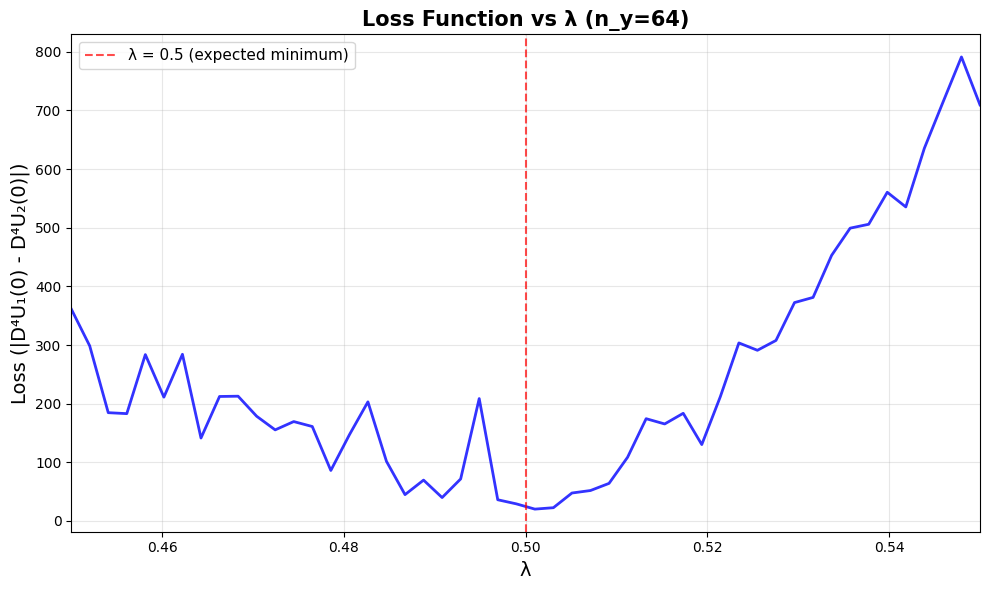
\includegraphics[width=0.7\textwidth]{images/loss_vs_lambda.png}
    \caption{Scalar objective $\mathcal{L}^{\mathrm{reg}}(\lambda)$ (see eq.~\eqref{eq:inference_loss}) as a function of $\lambda$. The sharp dip at $\lambda \approx 0.5$ indicates the location where the solution becomes smooth and the fourth-derivative jump vanishes.}
    \label{fig:loss_vs_lambda}
\end{figure}

\subsection{Inferring $\lambda$: numerical results}\label{subsec:inference_numerical_results}

In this section, we present the results of applying the nested optimization strategy to infer the parameter $\lambda$. As in Section~\ref{subsec:fixed_l_numerical_results}, we use $n_y = 64$ collocation points (see Remark~\ref{rmk:n_y-selection}). We initialize the Nelder--Mead outer optimization from $20$ random values of $\lambda$ sampled uniformly from the interval $[0.45, 0.55]$. Table~\ref{tab:nelder_mead_results} summarizes the results of a single run. We can see the Nelder--Mead optimization terminated successfully for all 20 initial values, requiring between 29 and 34 iterations and between 72 and 88 loss evaluations, which demonstrates the tractability of this formulation. Further, the recovered parameter value, $\lambda = 0.49915829$, lies within $8.4 \times 10^{-4}$ of the true smooth-solution value $\lambda = 0.5$. These results highlight the effectiveness of the approach: despite the markedly non-convex loss landscape—evidenced by the broad range of final loss values (from approximately $0.07$ to $43$)—the Nelder--Mead method is able to identify the global minimizer.

The primary drawback of this nested optimization framework is its computational cost. As shown in Table~\ref{tab:nelder_mead_results}, each run required roughly 80 loss evaluations, resulting in a total of about $20 \times 80 = 1600$ evaluations. Thus, the nested strategy is approximately $1600$ times more expensive than the fixed-$\lambda$ optimization described in Section~\ref{subsec:fixed_l_numerical_results}.
\begin{table}[tbhp]
    \centering
    \begin{tabular}{lc}
        \toprule
        Metric & Value \\
        \midrule
        Number of Initial Values & 20 \\
        Successful convergences & 20 \\
        Final $\lambda$ value & 0.49915829 \\
        Error from true value ($\lambda = 0.5$) & $8.4 \times 10^{-4}$ \\
        \midrule
        Iterations: min/max/mean & 29 / 34 / 31.0 \\
        Loss evaluations: min/max/mean & 72 / 88 / 79.3 \\
        Final loss: min/max/mean & 0.065 / 42.813 / 7.2 \\
        \bottomrule
    \end{tabular}
    \caption{Summary of Nelder--Mead optimization results from 20 random 
    initializations in $[0.45, 0.55]$. Single run of Nelder--Mead optimization (see Section~\ref{subsec:inference_optimization}). The wide range of final function values (0.065 to 42.813) 
    reflects the non-convex nature of the loss landscape, yet we successfully
    recovered the global minimum near $\lambda = 0.5$.}
    \label{tab:nelder_mead_results}
\end{table}

\section{Conclusions}\label{sec:conclusions}
In this report, we developed a collocation-based framework for solving the
self-similar Burgers equation and for inferring the parameter $\lambda$ that
distinguishes smooth from non-smooth similarity profiles. The localized
Chebyshev method proved effective on each subinterval, accurately capturing both
smooth and cusp-like behavior near the origin. Combined with automatic
differentiation and a multigrid-style initialization strategy, this approach
yielded accurate solutions for fixed $\lambda$. Because direct joint optimization over $(\lambda, U)$ is severely
ill-conditioned--due largely to the instability of high-order differentiation
matrices--we adopted a nested strategy in which the fixed $\lambda$ problem is solved in each iteration of the outer optimization,
and $\lambda$ is then inferred by minimizing a scalar measure of the
fourth-derivative jump. Despite the non-convexity of this objective, the
derivative-free Nelder--Mead method reliably recovered the correct smoothing
parameter $\lambda = 0.5$ with several digits of accuracy. Overall, these results show that localized spectral discretization combined with
nested optimization offers a robust framework for studying self-similar blowup
profiles and identifying smoothness-determining parameters. 

Future directions
include extending the method to other discrete values of $\lambda$ that admit
smooth similarity solutions (including unstable blowups), examining regimes that
require detecting nonsmoothness in even higher derivatives, and applying the
approach to more complex nonlinear PDEs.

\begin{remark}[Code]
    All code used for the results in this report can be found at\\
    \url{https://github.com/ayang923/AM205-project}.
\end{remark}

\bibliographystyle{abbrv}
\bibliography{references}


\end{document}

